\chapter{Surface Treatment, Ornament, and Essential Visibility}

\section{Ornament Is Relative to a Question}

A surface treatment is anything done to the appearance of geometry without changing the geometry: a colour, a texture, a bump pattern, a gloss, a shading model. Chapter 9 showed that a presentation is adequate or not relative to a question. The same holds for the treatments applied within a presentation. A feature of a surface is \emph{ornament relative to a question} when removing it changes the answer a reading procedure gives by no more than the tolerance $\varepsilon$ of Chapter 9, and it is \emph{essential} to that question when removing it changes the answer by more. The definition is operational. It can be tested by rendering the scene with and without the feature, applying the same reading procedure to both images, and comparing the answers. And it is relative: a wood grain on a floor is ornament for the question of where the entrance is and may be essential for the question of whether the floor is timber.

Ornament is not worthless, and the point of the definition is not to remove it. The point is to know what each treatment costs and what it buys, so that a figure carries the ornament its purpose can afford. A treatment can also cost something that is not decoration at all. A noise pattern has no information about the plinth, and it can still damage a reader's ability to find the plinth. This chapter measures that damage in a simple case, shows that its onset can be predicted from the colours alone, reports the cost in render time, which proved undetectable, and shows what a shading model contributes beyond colour.

\section{A Reading Task and a Noise Pattern}

The task is to find the plinth in an oblique view of the habitat of Chapter 9, with the east entrance. The reading procedure assigns each pixel to the nearest of four reference colours (plinth, floor, wall, background), measuring distance in the CIE Lab colour space, in which Euclidean distance approximates perceived colour difference. The distance between two colours in Lab is written $\Delta E$. The plinth is scored against a mask produced by rendering the same view with flat identity colours, and the score is the intersection over union of the pixels the procedure calls plinth with the pixels that are plinth. Precision is the share of called pixels that are right, and recall the share of true pixels that are called.

The ornament is a procedural noise pattern on the floor. A Noise Texture node, fed with object coordinates, is rescaled by a Map Range node and drives a Mix node between two tones of the floor colour, one darker and one lighter than the floor's base colour by a relative amplitude $a$. At $a=0$ the floor is flat, and at larger $a$ it is a speckle whose average tone stays at the base colour. The materials are emissive, so the pixel colours are the assigned colours, and the experiment isolates the effect of the pattern from the effect of lighting. The script is \texttt{ornament.py}.

Three plinth colours were used. The \emph{distinct} plinth is the blue of Chapter 7's palette, at $\Delta E=58.1$ from the floor's base colour. The other two are the floor colour scaled up in tone, by $1.15$ and by $1.45$, so that they have the same hue as the floor and differ in lightness only; their distances from the floor colour are $\Delta E=8.0$ and $23.8$. The tonal plinths are the hard case, because the noise pattern moves floor pixels along exactly the line that joins the floor colour to the plinth colour.

\section{What the Pattern Costs}

\begin{center}
\begin{tabular}{rrrr}
\toprule
Amplitude $a$ & sd of floor $L^*$ & IoU, $\Delta E=8.0$ & IoU, $\Delta E=23.8$\\
\midrule
0.00 & 0.00 & 1.000 & 1.000\\
0.10 & 2.14 & 0.447 & 1.000\\
0.20 & 4.22 & 0.123 & 1.000\\
0.35 & 7.15 & 0.073 & 0.249\\
0.50 & 8.10 & 0.060 & 0.106\\
\bottomrule
\end{tabular}
\end{center}

The blue plinth at $\Delta E=58.1$ was found with an intersection over union of $1.000$ at every amplitude, so for it the pattern is ornament in the sense defined above. For the two tonal plinths the pattern is not ornament: it takes the score from $1.000$ to $0.447$ at $a=0.10$ for the closer colour, and from $1.000$ to $0.249$ at $a=0.35$ for the other. In every case recall stayed at $1.000$ and precision equalled the score. The reading procedure never missed the plinth, because the plinth's colour was exact, and the entire loss came from floor pixels that the noise made closer to the plinth colour than to the floor colour. Figure 10.1 shows the case $\Delta E=23.8$ at three amplitudes, with the reading below each image.

\begin{figure}[ht]
\centering
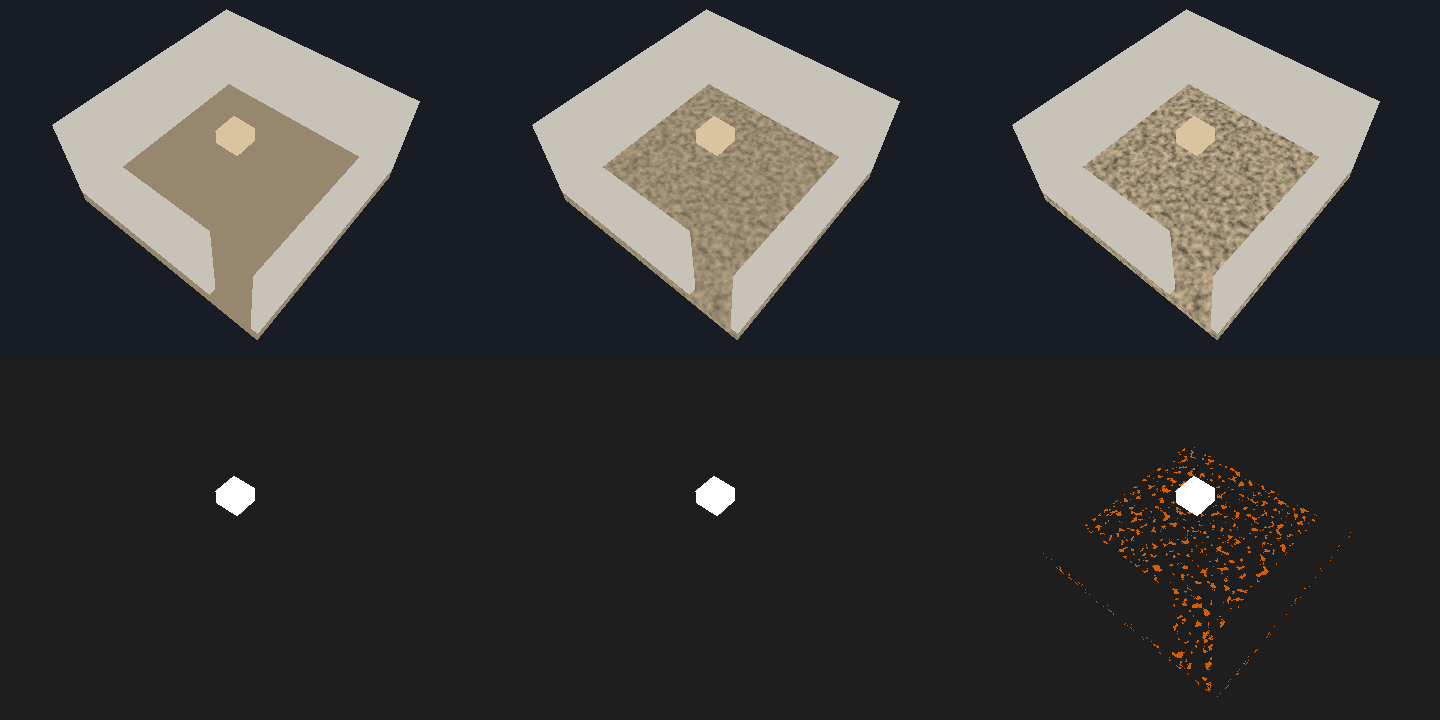
\includegraphics[width=\textwidth]{figs/fig10_ornament.png}
\caption{A plinth $1.45$ times the floor colour under floor ornament of amplitude $0$, $0.2$, and $0.35$ (top, left to right), and the nearest-colour reading of each (bottom). White marks plinth pixels found and orange marks floor pixels wrongly called plinth. At $a=0.2$ the reading is still exact, and at $a=0.35$ about three quarters of the pixels it calls plinth are floor.}
\end{figure}

The onset is predictable from the colours. The pattern moves a floor pixel as far as $a$ times its colour toward the plinth, and the reading procedure calls a floor pixel plinth when it has moved past the midpoint of the two colours. If the plinth is the floor colour multiplied by $s$, the midpoint is at $1+(s-1)/2$, and errors can begin when $a$ exceeds about $(s-1)/2$. For $s=1.15$ this is $0.075$ and the first failure was at $a=0.10$, the smallest amplitude tried above zero. For $s=1.45$ it is $0.225$, and the score was still $1.000$ at $0.20$ and had fallen at $0.35$. The rule is a first estimate: it works in sRGB scaling while the reading works in Lab, the pattern's extreme tones are reached only where the noise saturates, and the share of pixels beyond the midpoint depends on the pattern's distribution, so the rule says where errors begin and not how many there are. It is nevertheless the form of the useful statement, which is a relation between the spread of the ornament and the separation of the colours that carry the information.

The finding is specific to the reading procedure. A procedure that used shape, such as requiring a connected region of roughly the plinth's size, would tolerate much more noise, and a human reader's performance is unlikely to collapse as abruptly as a nearest-colour classifier. The measurement shows what a plain colour classifier needs, and a reader or a script that has a better procedure has less need of colour separation. Colour separation is cheap to provide and does not depend on the reader's skill, which is a reason to keep it when the figure must be read by an unknown reader.

\section{What the Pattern Costs in Time}

Chapter 8 measured render cost against samples and pixels, and it is natural to ask whether the pattern adds to it. A flat floor and a noise floor of amplitude $0.35$ were each rendered three times at $960\times720$ and $16$ samples, after a warm-up. The flat floor took $5.4$, $11.3$, and $10.8$ seconds and the noise floor $4.3$, $10.7$, and $10.9$ seconds. The runs with identical settings differed by a factor of two, so any difference attributable to the pattern is far below the scatter of the measurement, and no cost was detected. The pattern is a few nodes evaluated per pixel, and in this software-rendered configuration the fixed per-frame cost of Chapter 8 dominates. The conclusion is limited to this configuration and this scale. It does not say that textures are free on a graphics card with a large image, or in an animation of many frames, where a small per-pixel cost multiplies.

\section{What a Shading Model Adds}

The flat emissive materials used above erase one thing the plinth has, which is its form. In the flat render the plinth's mask contains a single colour, one distinct value in $1042$ pixels, with $L^*=46.0$, so the box looks like a hexagon. Rendered again with diffuse materials under ambient light and one sun lamp, the same mask contained six distinct colours of which three had at least twenty pixels, at $L^*=29.6$, $36.1$, and $36.2$. A shading model therefore separates the top of the plinth from its sides by $6.5$ units of $L^*$ and does not separate the two visible sides from each other, which differ by $0.1$. For the question of where the plinth is, the shading is ornament, because the reading above found it with a score of $1.000$ either way. For the question of whether the object is a solid box, the shading is essential, because without it the image contains nothing that says so. The two sides that are indistinguishable show a further point: a shading model gives information only where the light makes surfaces differ, and a light placed so that two faces receive the same illumination is a light that discards the distinction between them.

\section{A Rule for Choosing}

The measurements suggest a procedure for deciding how much surface treatment a figure should carry. List the questions the figure is meant to answer, and for each, write the colour or tone difference that carries its answer. Keep the separation between those colours larger than the spread of any ornament that will share their region of the image, using a relation such as $a<(s-1)/2$ as a first estimate and a rendered test as a confirmation. Then test whether each treatment is ornament or essential by removing it and applying the reading procedure, and keep the essential ones. What remains is a figure whose ornament was chosen, and whose cost is known to be small for the questions asked, and whose omission would not have changed what the reader can recover. The costs that were found are on the reader's side and not the renderer's, and that is why they deserve a measurement and not an assumption.

\begin{exercise}[10.1: Move the threshold]
Choose a plinth colour with $s=1.30$ and predict the amplitude at which the nearest-colour reading begins to fail, using $(s-1)/2$. Then measure the score at amplitudes $0.05$ to $0.30$ in steps of $0.05$ and report how close the prediction was.
\end{exercise}

\begin{exercise}[10.2: A better reader]
Add a second reading procedure that requires a candidate region to be connected and to contain between $500$ and $2000$ pixels, and repeat the measurement for the plinth with $\Delta E=8.0$. State the amplitude at which the new procedure fails, and say what it assumes about the plinth that the nearest-colour procedure did not.
\end{exercise}

\begin{exercise}[10.3: Ornament for a different question]
Choose a question for which a floor pattern is essential, such as whether the floor is made of a material with visible grain, and write a reading procedure and an ablation test for it. Show that the pattern is ornament for the plinth question and essential for yours.
\end{exercise}

\begin{exercise}[10.4: Lights that merge faces]
Find a direction for the sun lamp at which the top and sides of the plinth have the same $L^*$ to within $0.5$, and report what the image of the plinth then shows. State the lesson for a figure that must show form.
\end{exercise}
